% Document class and font size
\documentclass[a4paper,10pt]{extarticle}

% Packages
\usepackage[utf8]{inputenc} % For input encoding
\usepackage{geometry} % For page margins
\geometry{a4paper, margin=0.75in} % Set paper size and margins
\usepackage{titlesec} % For section title formatting
\usepackage{enumitem} % For itemized list formatting
\usepackage{hyperref} % For hyperlinks
\usepackage{kotex}
\usepackage{graphicx}
\usepackage{array}
\usepackage{longtable}

% Formatting
\setlist{noitemsep} % Removes item separation
\titleformat{\section}{\large\bfseries}{\thesection}{1em}{}[\titlerule] % Section title format
\titlespacing*{\section}{0pt}{\baselineskip}{\baselineskip} % Section title spacing
\graphicspath{{pictures}}

% Begin document
\begin{document}
% Disable page numbers
\pagestyle{empty}
% Enable page numbers
% \pagenumbering{arabic}

% Header

% \begin{minipage}{\textwidth}

\begin{minipage}{0.1\textwidth}
	\begin{flushleft}
		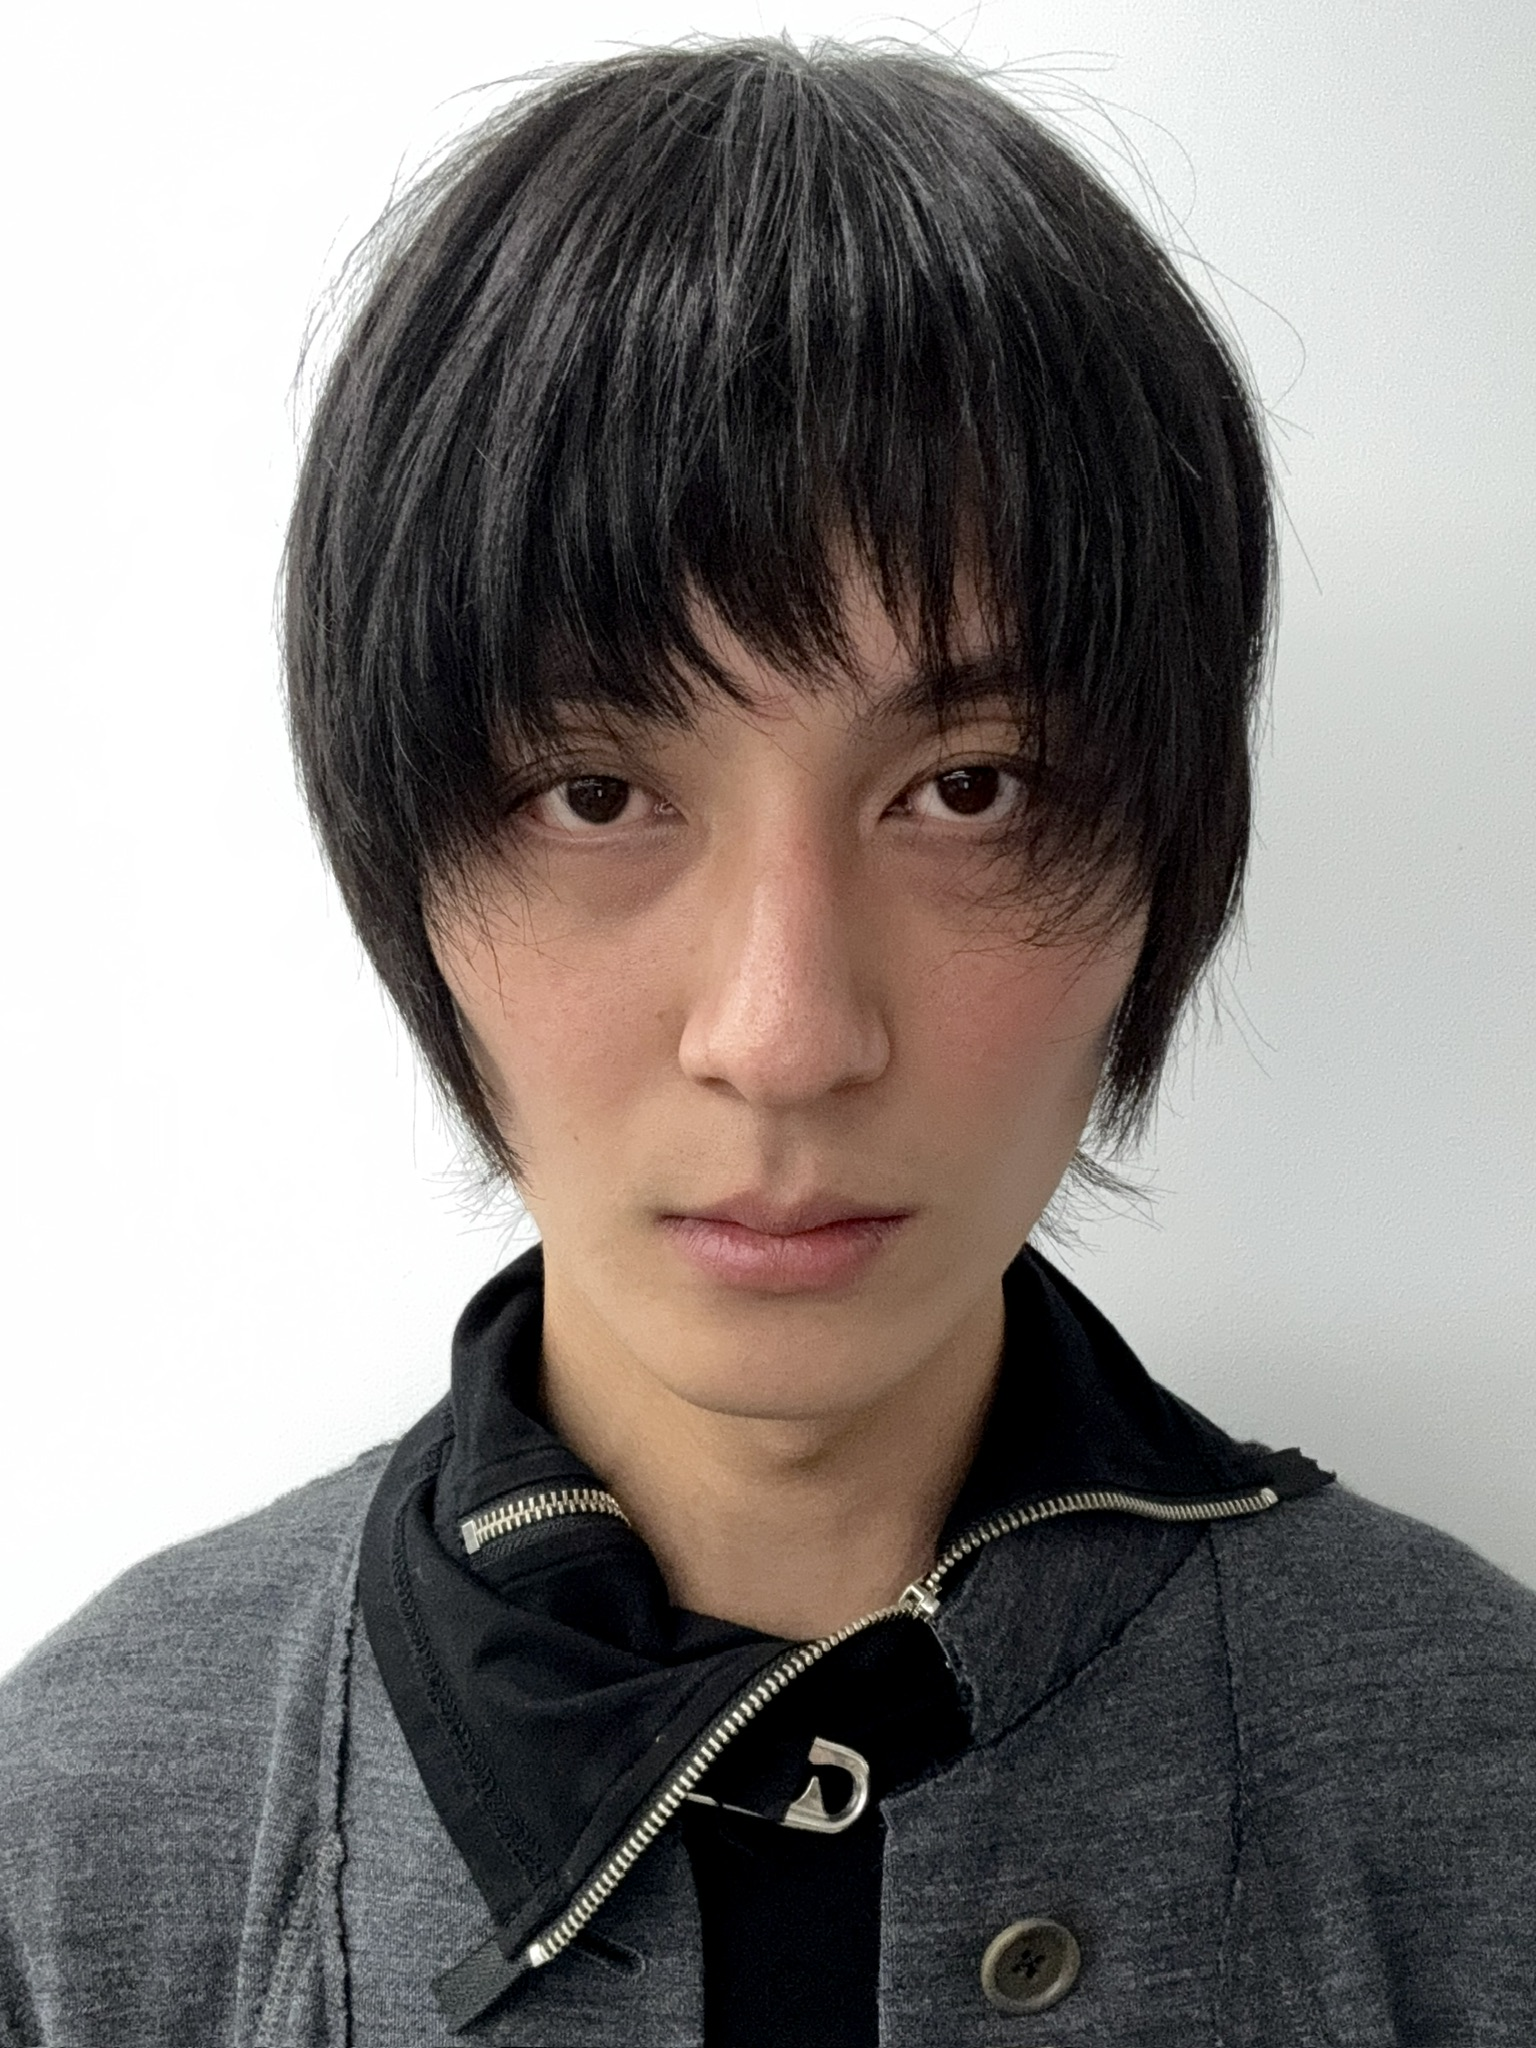
\includegraphics[height=3.5cm]{photo_dlicense.jpeg}
	\end{flushleft}
\end{minipage}
\hfill
\begin{minipage}{0.7\textwidth}
	\begin{flushright}
		\textbf{\Large Hyeonbeen Lee} % Name
		\newline\newline
		\begin{tabular}{rl}
			\textbf{Mobile: }         & \href{tel:+82-10-6236-4693}{+82-10-6236-4693}                                                                 \\
			\textbf{EMail: }          & \href{mailto:edward.hyeonbeen.lee@gmail.com}{edward.hyeonbeen.lee@gmail.com}                                  \\
			\textbf{GitHub: }         & \href{https://github.com/hyeonbeenlee}{github.com/hyeonbeenlee}                                               \\
			% \textbf{Instagram: } & \href{https://www.instagram.com/leehyeonbeen}{@leehyeonbeen}                                         \\
			\textbf{LinkedIn: }       & \href{https://www.linkedin.com/in/hyeonbeen-lee-239500286/}{linkedin.com/in/hyeonbeen-lee-239500286}          \\
			\textbf{Google Scholar: } & \href{https://scholar.google.com/citations?user=TiduRxoAAAAJ}{scholar.google.com/citations?user=TiduRxoAAAAJ} \\
		\end{tabular}
		% \end{center}
	\end{flushright}

\end{minipage}
% \end{minipage}


% Education Section
\newcolumntype{L}{>{\raggedright\arraybackslash}m{3.5cm}}
\newcolumntype{R}{>{\centering\arraybackslash\small}m{4cm}}
\renewcommand*{\arraystretch}{1.5}
\noindent
\section*{PERSONAL INFORMATION}
\begin{center}
	\vspace*{-0.8cm}
	\noindent
	\begin{longtable}{LRLRLR}
		\textbf{Legal Name:}       & Hyeonbeen Lee                                                                            & \textbf{Date of birth:}     & July 4th, 1996                                                       \\
		\hline
		\textbf{Nationality:}      & Republic of Korea (South)                                                                & \textbf{Address:}           & 6-3, Hoenamu-ro 39gil, Yongsan-gu, Seoul, South Korea                \\
		\hline
		\textbf{Military service:} & Honorably discharged,\linebreak Marine Corps Sergeant {\small (May 2017$\sim$Feb. 2019)} & \textbf{Research interest:} & Time series forecasting, Reinforcement learning, Sequential decision \\
		\hline
	\end{longtable}
\end{center}

% Education Section
\section*{EDUCATION}
\noindent
\textbf{Banpo High School}, Science-specialized Track \hfill Mar. 2012 | Feb. 2015
\newline
\textbf{Kyung Hee University}, Dept. of Mechanical Engineering \hfill Mar. 2015 | Feb. 2022\\ % University name and location
Bachelor of Engineering (Supervisor: Shin-kyu Jeong, Jin-gyun Kim)\hfill GPA(Major): 3.84/4.5, GPA: 3.87/4.5\\ % Degree and GPA
Thesis: \textit{{\small `Data-driven aerodynamic coefficient prediction using}}\\
\hspace*{1.3cm}\textit{{\small deep neural
			network and PARSEC airfoil parameterization'}}
\newline
\textbf{Kyung Hee University}, Dept. of Mechanical Engineering \hfill Mar. 2022 | Feb. 2024\\ % University name and location
Master of Engineering (Supervisor: Jin-gyun Kim) \hfill GPA: 4.33/4.5\\ % Degree and GPA
Thesis: \textit{{\small `Composite neural network with differential propagation}}\\
\hspace*{1.3cm}\textit{\small{for modeling impulsive nonlinear dynamic systems'}}

\section*{SKILLS}
\begin{itemize}
	\item \textbf{Programming: }Python, Docker, Linux, Git, \LaTeX, MATLAB, C\#, C++, ROS
	\item \textbf{ML and data analysis:} PyTorch, TensorBoard, Pandas, OpenCV, Torchvision
	      \begin{itemize}
		      \item \textit{Expertised at handling \underline{sequential data and models}}
	      \end{itemize}
	\item \textbf{English: }Speaks in native level
	\item \textbf{Japanese: }Speaks in intermediate level
\end{itemize}

\section*{CAREER}
\noindent
\textbf{8DIVISION}, Main Store Staff \hfill Feb. 2024 | Present
\begin{itemize}
	\item Global fashion sales
	\item Modeling and styling
	\item Social media creative management
	\item Robotic process automation using Python Selenium
	\item Sales analysis using Python dataprocessing libs
\end{itemize}
\textbf{Freelance model}\hfill May 2024 | Present
\begin{itemize}
    \item \href{https://instagram.com/gyoureekim}{@gyoureekim} SS2025 fitting model for \href{https://instagram.com/londonfashionweek}{London Fashion Week}
    \item \href{https://instagram.com/san263_1}{@san263$\_$1} FW2024/SS2025 fitting model
    \item \href{https://instagram.com/8division}{@8division}, \href{https://instagram.com/8division_journal}{@8division$\_$journal} store fitting model
	\item \href{https://instagram.com/armed_dept}{@armed$\_$dept} FW2024 Lookbook
	\item Personal works with photographers: \href{https://instagram.com/chtewon}{@chtewon}, \href{https://instagram.com/wyw_kiki98}{@wyw$\_$kiki98}, \href{https://instagram.com/leeejaehoon}{@leeejaehoon}, \href{https://instagram.com/jngsnghn}{@jngsnghun}
	\item Magazines: \href{https://instagram.com/pap_magazine}{@pap$\_$magazine}, \href{https://instagram.com/prism.mag}{@prism.mag}
\end{itemize}


% Experience Section
\section*{PUBLICATIONS}
\noindent
\begin{enumerate}[leftmargin=.5cm]
	\item \href{https://www.google.com/url?sa=t&rct=j&q=&esrc=s&source=web&cd=&cad=rja&uact=8&ved=2ahUKEwij36zWpNKCAxXMMEQIHSBfBMUQFnoECBEQAQ&url=https%3A%2F%2Fwww.sciencedirect.com%2Fscience%2Farticle%2Fpii%2FS1738573323003492&usg=AOvVaw1zj_G3k5c77uhMNnmu0EEC&opi=89978449}{S. Han, G.E. Jeong, \textbf{H. Lee}, W.S. Choi, J.G. Kim, “Multi-body dynamics model for spent nuclear fuel transportation system under normal transport test conditions”, \textit{Nuclear Engineering and Technology (Q1, JCR-IF Top 3.5\% in Nuclear Science \& Technology)}, 55(11), 4125-4133.}
	\item \href{https://www.sciencedirect.com/science/article/pii/S0021999123006733?casa_token=ARUkhI8XI8YAAAAA:wTzCIauJvSlonWw-J-SlAFqPX6NZRQS-qBX59l4YN5O3caEppoglU0duVmMkZYf4nWYd7tm_D_E}{\textbf{H. Lee}, S. Han, H.S. Choi, J.G. Kim (2023). “cNN-DP: Composite neural network with differential propagation for impulsive nonlinear dynamics”, \textit{Journal of Computational Physics (Q1, JCR-IF Top 4.5\% in Physics, Mathematical)}, 112578.}
	\item \textbf{H. Lee}, J. Han, T. Yeo, J.G. Kim. “Stochastic Fourier Transformer for interpretable real-time real-world robot force forecasting”, in preparation.
\end{enumerate}

% Experience Section
\section*{PROJECTS}
\noindent
\newcolumntype{L}{>{\raggedright\arraybackslash}m{3.6cm}}
\newcolumntype{R}{>{\raggedright\arraybackslash}m{13.2cm}}
\vspace*{-.5cm}
\begin{longtable}{LR}
	{Mar. 2022 | Oct. 2024} & Deep-learning based reaction force and torque prediction model development for underwater ground cutting robot using experimental measurements and dynamic simulation data, Korea Research Institute of Ships and Ocean Engineering (KRISO). (\href{https://github.com/hyeonbeenlee/TimeSeriesSeq2Seq}{github.com/hyeonbeenlee/TimeSeriesSeq2Seq}) \\
	{Nov 2021 | Jan. 2024}  & cNN-DP: Composite neural network with differential propagation for impulsive nonlinear dynamics, Modeling \& Simulation Lab. (\href{https://github.com/hyeonbeenlee/cNN-DP}{github.com/hyeonbeenlee/cNN-DP})                                                                                                                                       \\
	{Sep. 2021 | Jan. 2024} & Metamodel generation and evolution procedures for flexible multibody dynamics, FunctionBay Inc.                                                                                                                                                                                                                                                    \\
	{Mar. 2023 | Jun. 2023} & Segment Anyone: Fine-tuned Segment-Anything-Model (SAM) for human-collaborative robots, Kyung Hee University Dept. of Artifical Intelligence. (\href{https://github.com/hyeonbeenlee/segment-anything-fine-tuning}{github.com/hyeonbeenlee/segment-anything-fine-tuning})                                                                          \\
	{Dec. 2022 | Jun. 2023} & RecurDyn Automation using Python, Modeling \& Simulation Lab. (\href{https://github.com/hyeonbeenlee/RecurDynPython}{github.com/hyeonbeenlee/RecurDynPython})                                                                                                                                                                                      \\
	{Sep. 2021 | Oct. 2022} & Development of ground·sea transportation test simulation model using multibody dynamics and DNN-based metamodel, Korea Atomic Energy Research Institute (KAERI).                                                                                                                                                                                   \\
\end{longtable}

% Experience Section
\section*{CONFERENCES}
\noindent
\newcolumntype{L}{>{\raggedright\arraybackslash}m{3.4cm}}
\newcolumntype{R}{>{\raggedright\arraybackslash}m{13.2cm}}
\vspace*{-.5cm}
\begin{longtable}{LR}
	{Jun. 9 2024 \linebreak Madison, Wisconsin, USA} & J. Han, J.B. Han, S.S. Kim, M.H. Kim, Y.H. Kim, \textbf{H. Lee}, J.G. Kim, T.K. Yeu. “Digital twin model of underwater construction robot for real-time grinding simulation”, 7th International Conference on Multibody System Dynamics.                                  \\
	{Nov. 1 2023 \linebreak Incheon, South Korea}    & \textbf{H. Lee}, J. Han, T. Yeo, J.G. Kim. “Real-time multi-horizon reaction force forecasting of ocean robot using interpretable Transformer”, Annual Conference, Korean Society of Mechanical Engineers (Oral Presentation).                                            \\
	{May 18 2023 \linebreak Busan, South Korea}      & \textbf{H. Lee,} S. Han, H.S. Choi, J.G. Kim. “Meta-modeling of nonlinear impulsive dynamics using composite neural network model with differential propagation”, Conference on Engineering Reliability, Korean Society of Mechanical Engineers (Oral Presentation).      \\
	{Mar. 23 2023 \linebreak Jeju, South Korea}      & \textbf{H. Lee,} S. Han, H.S. Choi, J.G. Kim. “Meta-modeling of nonlinear impulsive dynamics using composite neural network model with differential propagation”, Conference on Dynamics and Control, Korean Society of Mechanical Engineers (Oral Presentation).         \\
	{Feb. 16 2023 \linebreak  Austin, Texas, USA}    & \textbf{H. Lee,} S. Han, H.S. Choi, J.G. Kim. “Composite neural network framework for modeling impulsive nonlinear dynamic responses”, 41th International Modal Analysis Conference (IMAC) (Oral Presentation).                                                           \\
	{Dec. 4 2022 \linebreak Jeju, South Korea}       & \textbf{H. Lee}, S. Han, G.E. Jeong, J.G. Kim. “Development of multibody dynamics trailer model using normal transportation test data and DNN based surrogate model generation”, Fall conference, Korean Society for Noise and Vibration Engineering (Oral Presentation). \\
\end{longtable}

% Skills Section
\section*{AWARDS AND CERTIFICATES}
\begin{itemize}
	\item \textbf{New TEPS:} 513/600 (equivalent to TOEIC 980/990) \hfill No.0111736, Valid, May 13 2023

	\item \textbf{OPI English:} AH (Advanced High) \hfill 2A7617334333, Valid, Nov. 14 2023
	\item \textbf{RA Scholarship (80\% tuition)} \hfill Kyung Hee University, Sep. 01 2023
	\item \textbf{Exellence Paper Award} \hfill Korean Society of Mechanical Engineers, No.2023-083, Aug. 25 2023
	\item \textbf{RA Scholarship (80\% tuition)} \hfill Kyung Hee University, Mar. 01 2023
	\item \textbf{RA Scholarship (80\% tuition)} \hfill Kyung Hee University, Sep. 01 2022
	      % \item \textbf{행정조교 장학금} \hfill 경희대학교 대학원, 수혜년월: 2022.09 | 2024.02
	\item \textbf{Excellence Scholarship (Full tuition)} \hfill Kyung Hee University, Mar. 01 2021
	\item \textbf{TOEIC:} 925/990 \hfill No.605083, Expired, Nov 25 2018
\end{itemize}

% Experience Section
% \section*{사회경험}
% \noindent
% \textbf{맥도날드 서울교대점} 고객응대, 주방보조, 계산 \hfill 2014.11 - 2015.02\\
% \textbf{육회한연어 수원영통점} 서빙, 주방보조, 계산 \hfill 2016.02 - 2016.06\\
% \textbf{슈펜 가로수길점} 외국인 고객응대, 물류창고정리 \hfill 2016.06 - 2016.09\\
% \textbf{오늘 와인한잔 수원역점} 서빙, 주방보조 \hfill 2016.09 - 2016.12\\
% \textbf{아이리스 BAR} 서빙, 주방보조, 고객응대 \hfill 2019.03 - 2019.06\\
% \textbf{대명GEC} 삼성전자 화성사업장 케이블 배선작업 \hfill 2019.07 - 2019.08\\

% Experience Section
\section*{MISCELLANEOUS}
\textbf{Representative Administrative Assistant} \hfill Kyung Hee University, Sep 2022 | Present\\
\textbf{Seminar: IAS18 Workshop\&Tutorials} \hfill {\small Intl. Conference on Intelligent Autonomous Systems}, Jul 2023\\
\textbf{Seminar: AI Summer School 2022} \hfill Korean Society of Mechanical Engineers, Aug 2022\\
\textbf{Teaching Assistant (System Dynamics)} \hfill Modeling \& Simulation Lab, Mar 2022 - Jun 2023\\
\textbf{Seminar: AI Summer School 2021} \hfill Korean Society of Mechanical Engineers, Aug 2021\\
\textbf{Seminar: AI, Data Driven Models\&ML} \hfill {\small National Agency Finite Element Methods and Standard}, Apr 2021\\
\textbf{Undergraduate Research Internship} \hfill Modeling \& Simulation Lab, Jan 2021 | Feb 2022\\
\textbf{48th Student Council} \hfill Kyung Hee University College of Engineering, Feb 2019 | Jan 2020\\
\textbf{R.O.K.-U.S. Combined Marine Corps Interpreter} \hfill 1st Marine Div., ROKMC, Sep 2017 | Feb 2019\\
% End document
\end{document}